\section{概要}

ソフトウェアエンジニアや研究者には、マニュアルや論文などの技術文書を書く機会が多く存在する。
記述される技術文書は ``規約'' にしたがって記述するという共通の特徴を持つ。ここで文書の規約は文書の執筆者が従うべきルールである。

一般的に規約は集団で文書を作成する際にメンバが従うべき共通のルールとして使用される。
個人で文書を記述する際にも、文書全体が一貫した記述になるために策定されることがある。
規約には文の長さ、利用する句読点の種類 (半角全角など) 、文書中で利用する技術用語の選択などがある。

規約は文書を作成する組織ごとに大きく異なる。たとえば、アルゴリズムをアルファベットで記述する組織もあれば、
カタカナに変換して記述する組織も存在する。どちらを採用しても大きな問題はないが、
規約が混在してしまうと文書の可読性が低下したり、印象を損ねるおそれがある。

そのため、規約の遵守は重要な課題の一つと言える。本稿ではドキュメントが規約に従って記述されているか
自動検査するツール RedPen~\cite{redpen}\cite{ito15repden} について解説する。

次節でドキュメントを自動で検査するツール (ドキュメント検査ツール) について紹介する。
その後 RedPen の特徴と拡張方法について解説する。

% @suppress InvalidSymbol LongKanjiChain
\section{背景: ドキュメント検査ツール}
これまでにドキュメント検査ツールは提案されてきた。
株式会社ジャストシステムが提供している校正支援ツール Just Right!~\cite{justright} は
文の誤り検査、用語基準、表現など多くの機能を提供している。
ただし Just Right! は商用製品のため無料で利用できない。

また、自動で文書検査するツールに日本語表現法開発プロジェクト (PaWeL) が公開している
 Tomarigi~\cite{tomarigi}~\cite{tomarigi-paper} は無料で利用できる文書の自動検査ツール
や``Chantokun''~\cite{chantokun} がある。しかしこれらのツールはコマンドラインでの利用ができない。
そのため、これらのツールは Git などのバージョン管理システムや他のコマンドラインツールと
組み合わせて利用できない。また、ユーザや所属組織によって異なる規約にあわせてルールを
修正できないという問題がある。

文法誤りの検出だけではなく訂正を行う研究に水本ら~\cite{mizumoto12english} による英文法の自動誤り
訂正を行った研究がある。しかし、提案された手法は一般的に利用できる形では配布されていない。

さらに本格的なドキュメントはマークアップ言語を利用して記述されるが、ほとんどのドキュメント検査ツール
はマークアップ言語に対応していない。そのため上記のツールを利用してドキュメントを検査するには、前もって
ドキュメントからマークアップタグを削除する必要がある。

現在、マークアップ言語にも対応したドキュメント検査ツールには RedPen と textlint~\cite{textlint} の二つが存在する。
本稿では、その中の RedPen について詳しく解説する。

% @suppress CommaNumber ParagraphNumber
\section{RedPen の特徴}

以下 RedPen の主な特徴である。

\begin{description}
\item[{\bf 拡張性}]
  プラグインシステムを提供している。ユーザは Java もしくは JavaScript でパターンを記述して機能を追加できる。

\item[{\bf マークアップ言語 (フォーマット) への対応}]
  現状では平文、Markdown、Textile (Wiki記法) 、AsciiDoc、LaTeX、Re:VIEW に対応している。

\item[{\bf 複数の言語に対応}]
  日本語や英語でのみ動作する機能があるが (カタカナスペル検査など) 、多くの RedPen が提供する機能は任意の言語で記述された文書に対して動作する。

\item[{\bf 設定の柔軟さ}]
  RedPen で利用する規約は単一の設定ファイルですべて記述される。設定ファイルは XML フォーマットで、ユーザは検査したい項目を設定ファイルに追加する。図~\ref{fig:conf} は RedPen の設定例である。設定ファイルの validators ブロックに必要な機能 (validaotor) を追加する。図~\ref{fig:conf} では、SentenceLength (文の最大長) や InvalidSymbol (利用するシンボル) などの機能が追加されている。

\item[{\bf UI と REST API}]
  RedPen はコマンドラインだけでなく、Web UI と実用的な REST API を提供している。

\item[{\bf エディタ}]
  RedPen をエディタ上で利用できるパッケージが存在する。
  現在 RedPen を利用できるエディタには Atom、Emacs、Vim、IntelliJ IDEA がある。
  各エディタは共通の設定ファイルを利用できるため、執筆者は扱い慣れたエディタで文書検査ができる。
  図~\ref{fig:intellij-idea} は IntelliJ IDEA というエディタの RedPen パッケージが動作している様子である。
  RedPen パッケージでは、一部の問題をコマンド (ショートカットキー) で修正できる。画像では、半角スペースの問題
  をショートカットキーを通して修正している様子である。
\end{description}

\begin{figure}
  \scriptsize
  \small
  \begin{verbatim}
<validator-conf lang="en">
  <validators>
    <validator name="SentenceLength">
      <property name="max_len"
                value="150"/>
    </validator>
    <validator name="InvalidSymbol"/>
    <validator name="SpaceWithSymbol"/>
    <validator name="SectionLength"/>
  </validators>
</validator-conf>
  \end{verbatim}
  \normalsize
  \caption{RedPenの設定例}
  \label{fig:conf}
\end{figure}

\begin{figure*}[t]
  \begin{center}
    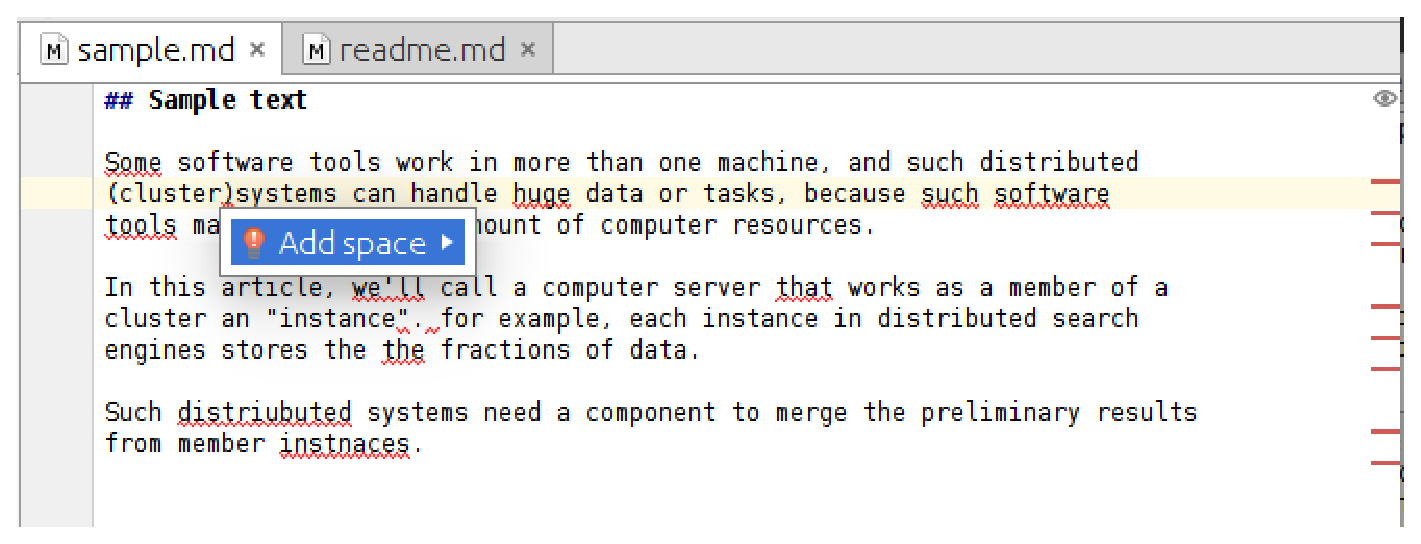
\includegraphics[width=15cm]{figs/quick-fix.eps}
    \caption{IntelliJ IDEA RedPen パッケージ}
    \label{fig:intellij-idea}
  \end{center}
\end{figure*}

\section{RedPen の拡張}
\label{sec:extension}
RedPen は数十個ほど文書検査で利用する機能を提供している。しかしそれでも、ユーザによっては必要な機能足りない場合がある。
そこで RedPen ではユーザが機能を自作できる環境 (プラグイン機構) を用意している。プラグインは Java と JavaScript で記述できる。
どちらで機能を作成しても問題ないが、JavaScript の方が手軽に作成できる。本節では JavaScript を利用した機能の作成方法をについて解説する。

機能を作成するには、validateSentence か validateSection 関数を実装する。
それぞれ、RedPen によりドキュメント内に存在する全ての文もしくは節が引数として適用される。
今回はサンプルとして、長すぎる漢字列を検知する機能を作成する。

\begin{figure}
  \scriptsize
  \small
  \begin{verbatim}
function validateSentence(sentence) {
    var pat = new RegExp("[\u4e00-\u9faf]{6,}", 'g');

    while (m = pat.exec(sentence.content)) {
      addError('長い熟語 "' + m[0] + '" (' +
              m[0].length + ') +
              が使われています。', sentence);
   }
}
  \end{verbatim}
  \normalsize
  \caption{長すぎる漢字列を検知する機能の実装例}
  \label{fig:js-validator}
\end{figure}

図~\ref{fig:js-validator} をみると、機能の実装は数行で実現できていることがわかる。
機能の作成では、はじめに漢字の連続が六回以上続いた場合にマッチする正規表現を作成している。
その後、各文についてが正規表現とマッチするかを判定している。
正規表現にマッチするとエラーを addError 関数で作成~\footnote{addError 関数は RedPen によって提供されているエラーを追加する関数} している。

\section{まとめ}
本稿では自動ドキュメント検査ツール RedPen を解説した。
具体的には RedPen の特徴を解説し、その後、利用方法および拡張方法について紹介した。
